
\documentclass[12pt, a4paper]{article}


%%%% Encodings

\usepackage[utf8]{inputenc} % encoding
\usepackage[english]{babel} % use special characters and also translates some elements within the document.

%%%% Misc

\usepackage{hyperref}       % Hyperlinks \url{url} or \href{url}{name}
\usepackage{parskip}        % \par starts on left (not idented)
\usepackage{tocbibind}      % Adds the bibliography to the table of contents (automatically)

% \usepackage[document]{ragged2e}  % Left-aligned (whole document)
% \begin{...} ... \end{...}   flushleft, flushright, center

%%%% Abstract

\usepackage{abstract}       % Abstract

% http://www.ctex.org/documents/packages/special/abstract.pdf
\renewcommand{\absnamepos}{flushleft} % \begin{abstract} \noindent ... \end{abstract}
\setlength{\absleftindent}{0pt}
\setlength{\absrightindent}{0pt}

%%%% Graphics

\usepackage{graphicx}
\graphicspath{ {./images/} } % directory to look up for graphics

% \begin{figure}[h]
%   \centering
%   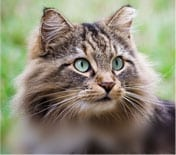
\includegraphics[scale=0.5]{cat}  % [width=\textwidth, height=4cm],
%   \caption{Example of a cat}
%   \label{fig:cat}
% \end{figure}

%%%% Math

\usepackage{amsmath}        % Math
\usepackage{amssymb}        % New symbols http://milde.users.sourceforge.net/LUCR/Math/mathpackages/amssymb-symbols.pdf
\usepackage{bm}             % $\bm{D + C}$

\usepackage{amsthm} % Math, \newtheorem, \proof, etc
% \begin{theorem}\label{t:label}  ...  \end{theorem}
% \begin{proof} ... \end{proof}
\theoremstyle{plain} % default
\newtheorem{theorem}{Theorem}[section]
\newtheorem{corollary}{Corollary}[theorem]  % Numering depends on the current section (instead of global)
\newtheorem{lemma}[theorem]{Lemma} % Shares numeration with theorem.
\theoremstyle{definition}
\newtheorem{definition}{Definition}[section]
\theoremstyle{remark}
\newtheorem*{remark}{Remark}

% Defines a new environment to write your or claim - proof
\newenvironment{claim}[1]{\par\noindent\underline{Claim:}\space#1}{}
\newenvironment{claimproof}[1]{\par\noindent\underline{Proof:}\space#1}{\hfill $\blacksquare$}

%%%% Code/Pseudo-code

\usepackage{minted} % Code listing
% \mint{html}|<h2>Something <b>here</b></h2>|
% \inputminted{octave}{BitXorMatrix.m}

%\begin{listing}[H]
  %\begin{minted}[xleftmargin=20pt,linenos,bgcolor=codegray]{haskell}
  %\end{minted}
  %\caption{Example of a listing.}
  %\label{lst:example} % You can reference it by \ref{lst:example}
%\end{listing}

\newcommand{\code}[1]{\texttt{#1}} % Define \code{foo.hs} environment

\usepackage[vlined,ruled]{algorithm2e} % pseudo-code http://tug.ctan.org/macros/latex/contrib/algorithm2e/doc/algorithm2e.pdf

%%%% Colors

\usepackage{xcolor}         % Colours \definecolor, \color{codegray}
\definecolor{codegray}{rgb}{0.9, 0.9, 0.9}
% \color{codegray} ... ...
% \textcolor{red}{easily}

%%%% Math

%\makeglossaries % before entries

%\newglossaryentry{latex}{
    %name=latex,
    %description={Is a mark up language specially suited
    %for scientific documents}
%}

% Referene to a glossary \gls{latex}
% Print glossaries \printglossaries

\usepackage[acronym]{glossaries} %

% \acrshort{name}
% \acrfull{name}
% \newacronym{foo}{arcshort}{acrfull}

\usepackage{enumitem}


\usepackage{fancyhdr}
\pagestyle{fancy}
\fancyhf{}
\rhead{AMMM}
\lhead{}
\rfoot{Page \thepage}

\title{%
  \vspace{-10ex}
  Algorithmic Methods for Mathematical Models \\
  \large{Assignment: Greedy Algorithms}
}
\author{%
  Arnau Abella \\
  \large{Universitat Polit\`ecnica de Catalunya}
}

\begin{document}

\maketitle

% \vspace{5ex}
\begin{enumerate}[label=(\alph*)]

  %%%%%%%%%%%%%%%%%%% a
  \item Specify the algorithm, including: i) the candidates; and ii) the greedy function $q()$. Specify $q()$ using mathematical notation and a short descriptive text.

  \textit{Note: Local Search included.}

    \begin{algorithm}[H]
      \SetAlgoLined
      \DontPrintSemicolon
      \SetKwInput{Input}{Input}
      \SetKwInput{Output}{Output}
      \Input{
        \begin{itemize}
          \item A set of offices $O$, each office $o$ requires $b_{0}$ PetaBytes ($10^{6}$ GB) of data storage
          \item A set of storage providers $D$, each storage provider $d$ has a capacity $k_{d}$ in PBs, a fixed cost $f_{d}$ and an additional cost $s_{d}$ per stored PB
        \end{itemize}
      }
      \Output{A set $w$ of assignments $\angles{d, O'}$
        where $d \in D$, $O' \subseteq O$, $|O'| \le 3$, $|w| \le 3$, $\bigcup\limits_{O'_{i} \in w} O'_{i} = O$ and $\bigcap\limits_{O'_{i} \in w} O'_{i} = \emptyset$
      }
      $w \leftarrow \emptyset$\;
      \ForAll{$o \in O$}{
        \tcc{$c_{min}$ is the cost of the minimal assignment\\
        $d_{u}$ is the storage provider to upgrade
        }
        $(c_{min}, d_{min}, d_{u}) \leftarrow argmin \{q(\angles{o, d}, w) | \ d \in D \}$\\
        \uIf{$c_{min} = \infty$}{\Return{$INFEASIBLE$}}
        \uElseIf(\tcc*[f]{update the assigned offices}){$d_{min} \in w$}{
          $O'' \leftarrow O'_{d_{min}} \cup \{ o \}$\\
          $w \leftarrow w \cup \{ \angles{ d_{min}, O''} \}$
        }
        \uElseIf(\tcc*[f]{add a new storage provider}){$|w| < 3 \land d_{u} = null$}{
          $w \leftarrow w \cup \{ \angles{ d_{min}, \{ o \}} \}$
        }
        \Else(\tcc*[f]{replace $d_{u}$ storage provider}){
          $w' \leftarrow w \setminus \{ d_{u} \}$\\
          $O'' \leftarrow \{ O'_{d_{u}} \cup \{ o \}\}$\\
          $w \leftarrow w' \cup \{ \angles{ d_{min}, O''} \}$
        }
      }
      \Return{$w$}
      \caption{Greedy Algorithm}
    \end{algorithm}

    \begin{figure}[H]
      \begin{align*}
        &q(\angles{o, d}, w) =
          \begin{cases}
              \infty & d \in w \land (|O'_{d}| = 3 \lor b_{o} > (k_{d} - \sum_{o' \in O'}b_{o'}))    \\
              b_{o}s_{d} & d \in w \land |O'_{d}| < 3 \land b_{o} \le (k_{d} - \sum_{o' \in O'}b_{o'})    \\
              q'(\angles{o, d}, w) & d \notin w \land |w| = 3 \\
              min (f_{d}+ b_{0}s_{d}, \ q'(\angles{o, d}, w)) & d \notin w \land |w| < 3
          \end{cases}\\
        &q'(o, d, w) = min \{ q'(o, d, d', w) | d' \in w \}\\
        &q'(o, d, d', w) =
          \begin{cases}
            \infty & |O'_{d'}| = 3 \lor b_{o} > (k_{d} - \sum_{o' \in O'_{d'}}b_{o'}) \\
            {\scriptstyle(f_{d}+s_{d}(b_{o} + \sum_{o' \in O'_{d'}}b_{o'})) - (f_{d'}+s_{d'}(b_{o} + \sum_{o' \in O'_{d'}}b_{o'}))} & |O'_{d'}| < 3 \land b_{o} \le (k_{d} - \sum_{o' \in O'_{d'}}b_{o'}) \\
          \end{cases}
      \end{align*}
      \caption{Cost function}
    \end{figure}

  %%%%%%%%%%%%%%% b
  \item Detail the decisions made in every iteration of the algorithm until a solution is obtained. For each iteration, compute the value of the proposed greedy function $q()$ for all the candidates.

  \textit{Note: this execution does not include the Local Search}.

    \begin{table}[H]
    \begin{tabular}{l|lllll}
    Office & \multicolumn{1}{l}{$d_{1}$} & \multicolumn{1}{l}{$d_{2}$} & \multicolumn{1}{l}{$d_{3}$} & \multicolumn{1}{l}{$d_{4}$} & $d_{5}$ \\ \hline

    q($o_{1}$)                    & \multicolumn{1}{l|}{500} & \multicolumn{1}{l|}{\cellcolor[HTML]{34FF34}380} & \multicolumn{1}{l|}{380} & \multicolumn{1}{l|}{890} & 700\\ \hline
    q($o_{2}$)                    & \multicolumn{1}{l|}{500} & \multicolumn{1}{l|}{\cellcolor[HTML]{34FF34}30} & \multicolumn{1}{l|}{380} & \multicolumn{1}{l|}{890} & 700\\ \hline
    q($o_{3}$)                    & \multicolumn{1}{l|}{500} & \multicolumn{1}{l|}{$\infty$} & \multicolumn{1}{l|}{\cellcolor[HTML]{34FF34}380} & \multicolumn{1}{l|}{890} & 700\\ \hline
    q($o_{4}$)                    & \multicolumn{1}{l|}{500} & \multicolumn{1}{l|}{$\infty$} & \multicolumn{1}{l|}{\cellcolor[HTML]{34FF34}130} & \multicolumn{1}{l|}{890} & 700\\ \hline
    q($o_{5}$)                    & \multicolumn{1}{l|}{500} & \multicolumn{1}{l|}{$\infty$} & \multicolumn{1}{l|}{\cellcolor[HTML]{34FF34}130} & \multicolumn{1}{l|}{890} & 700\\ \hline
    q($o_{6}$)                    & \multicolumn{1}{l|}{\cellcolor[HTML]{34FF34}500} & \multicolumn{1}{l|}{$\infty$} & \multicolumn{1}{l|}{$\infty$} & \multicolumn{1}{l|}{890} & 700\\ \hline
    q($o_{7}$)                    & \multicolumn{1}{l|}{\cellcolor[HTML]{34FF34}200} & \multicolumn{1}{l|}{$\infty$} & \multicolumn{1}{l|}{$\infty$} & \multicolumn{1}{l|}{890} & 700\\ \hline
    \end{tabular}
    \end{table}

\end{enumerate}

\end{document}
